\documentclass[journal]{IEEEtran}
\usepackage{graphicx}
\usepackage[outdir=./]{epstopdf}
\usepackage{subfigure}
\usepackage{hyperref}
\usepackage{booktabs}
\usepackage[table]{xcolor}
\usepackage{multirow}

\usepackage[utf8]{inputenc}
\usepackage[spanish, mexico]{babel}

%\usepackage{algorithm}
%\usepackage{algorithmic}
\usepackage{algorithmicx}
\usepackage{algorithm}
%\usepackage{ragged2e}
%\usepackage[utf8]{inputenc}
\usepackage{algpseudocode}% http://ctan.org/pkg/algorithmicx
%\floatname{algorithm}{Algoritmo}
\renewcommand{\listalgorithmname}{Lista de algoritmos}
\renewcommand{\algorithmicrequire}{\textbf{Entrada:}}
\renewcommand{\algorithmicensure}{\textbf{Salida:}}
\renewcommand{\algorithmicend}{\textbf{fin}}
\renewcommand{\algorithmicif}{\textbf{si}}
\renewcommand{\algorithmicthen}{\textbf{entonces}}
\renewcommand{\algorithmicelse}{\textbf{si no}}
\renewcommand{\algorithmicelsif}{\algorithmicelse,\ \algorithmicif}
\renewcommand{\algorithmicendif}{\algorithmicend\ \algorithmicif}
\renewcommand{\algorithmicfor}{\textbf{para}}
\renewcommand{\algorithmicforall}{\textbf{para todo}}
\renewcommand{\algorithmicdo}{\textbf{hacer}}
\renewcommand{\algorithmicendfor}{\algorithmicend\ \algorithmicfor}
\renewcommand{\algorithmicwhile}{\textbf{mientras}}
\renewcommand{\algorithmicendwhile}{\algorithmicend\ \algorithmicwhile}
\renewcommand{\algorithmicloop}{\textbf{repetir}}
\renewcommand{\algorithmicendloop}{\algorithmicend\ \algorithmicloop}
\renewcommand{\algorithmicrepeat}{\textbf{repetir}}
\renewcommand{\algorithmicuntil}{\textbf{hasta que}}
\renewcommand{\algorithmicprint}{\textbf{imprimir}} 
\renewcommand{\algorithmicreturn}{\textbf{devolver}} 
\renewcommand{\algorithmictrue}{\textbf{cierto }} 
\renewcommand{\algorithmicfalse}{\textbf{falso }} 


%%%%%%%%%%%%%%%%%%%%%%%%%%%%%%%%%%%%%%%%%%%%%%%%%%%%%%%%%%%%%%%%%
%% The following definitions are to extend the LaTeX algorithmic 
%% package with SWITCH statements and one-line structures.
%% The extension is by 
%%   Prof. Farn Wang 
%%   Dept. of Electrical Engineering, 
%%   National Taiwan University. 
%% 
\algnewcommand\algorithmicswitch{\textbf{switch}}
\algnewcommand\algorithmiccase{\textbf{case}}
\algnewcommand\algorithmicassert{\texttt{assert}}
\algnewcommand\Assert[1]{\State \algorithmicassert(#1)}%
\algdef{SE}[SWITCH]{Switch}{EndSwitch}[1]{\algorithmicswitch\ #1\ \algorithmicdo}{\algorithmicend\ \algorithmicswitch}%
\algdef{SE}[CASE]{Case}{EndCase}[1]{\algorithmiccase\ #1}{\algorithmicend\ \algorithmiccase}%
\algtext*{EndSwitch}%
\algtext*{EndCase}%
%% 
%% End of the LaTeX algorithmic package extension.
%%%%%%%%%%%%%%%%%%%%%%%%%%%%%%%%%%%%%%%%%%%%%%%%%%%%%%%%%%%%%%%%%


\usepackage{float}
\usepackage{mathpazo}
\begin{document}

% Corregir problemas de separación de palabras por guiones
%\hyphenation{op-tical net-works semi-conduc-tor}

\floatname{algorithm}{Pseudocódigo}
\title{Funcionamiento local de un dispositivo domótico, modulo de luces y aire acondicionado}

\author{Juanita~Hernández~López,~\IEEEmembership{Estudiante maestría,~LTI Cinvestav,}
        Rafael~Pérez~Torres,~\IEEEmembership{Estudiante doctorado,~LTI Cinvestav}.

	\thanks{Juanita Hernández López es estudiante de Maestría en Ciencias de la Computación en el Laboratorio de Tecnologías de Información del CINVESTAV, e-mail: jhernandez@tamps.cinvestav.mx.}
	\thanks{Rafael Pérez Torres es estudiante de doctorado en Ciencias de la Computación en el Laboratorio de Tecnologías de Información del CINVESTAV, email: rperez@tamps.cinvestav.mx.}
}

\markboth{Sistemas Embebidos, Noviembre~2014}%
{Hernández and Pérez: Sistemas embebidos}

\maketitle

\begin{abstract}
%\boldmath
Los sistemas embebidos (SE) son capaces de percibir su entorno, obtener información de éste y actuar en consecuencia para resolver un problema. 
Con este fin, los SE cuentan con un modelo formal que les permite abstraer los detalles del problema, creando una representación simplificada del mundo para así generar una solución.
Esta capacidad de adquisición de conocimiento del medio ambiente que les rodea les convierte en un elemento clave para el desarrollo de aplicaciones que enfrenten nuevos retos en distintas áreas de la investigación tales como el cómputo móvil, la aeronáutica, y la medicina.
En particular, la domótica representa una de las grandes áreas de desarrollo para los SE.

El presente documento propone la implementación de un SE que simula el comportamiento de un dispositivo domótico modular, controlando las luces y aire acondicionado en un una habitación.

\end{abstract}

\begin{IEEEkeywords}
Sistemas embebidos,  Lego NXT, Domótica.
\end{IEEEkeywords}

\section{Introducción}
\label{sec:introduccion}

La creciente presencia de SE en productos y servicios del mundo moderno ha permitido el desarrollo de distintas áreas de la ciencia y la tecnología.
Los SE desempeñan un papel importante no sólo en los dispositivos de electrónica de uso común, sino también en sistemas de seguridad crítica. 
Como consecuencia, existe especial interés en desarrollar herramientas que permitan crear aplicaciones sobre SE, creando un círculo virtuoso en el que las necesidades y características de las aplicaciones mejoran a los SE y viceversa.

Dichos sistemas están creciendo en popularidad al existir una gran variedad de aplicaciones que hasta cierto punto han logrado hacer nuestras vidas más dependientes de los mismos.
Se ha estimado que el 99\% \cite{Burns2005} de la producción mundial de microprocesadores se destina para su implementación en SE, siendo prácticamente invisibles para los consumidores.

Actualmente, los nichos de aplicación de los SE involucran elementos de seguridad crítica como controladores de dispositivos para aviones, automóviles, ferrocarriles, industria aeroespacial, salud y dispositivos médicos, comunicaciones, sistemas móviles y medio ambiente.
Sin embargo, el desarrollo de aplicaciones embebidas está entrando en nuevos dominios gracias a la disponibilidad de nuevos procesadores con mayores capacidades de cómputo, menor consumo de energía y un costo cada vez menor.
Una de las nuevas áreas donde los SE están jugando una participación medular es la domótica, la cual se refiere al conjunto de sistemas que enriquecen una vivienda mediante tecnología que responde a los objetivos del usuario en sus tareas comunes, de forma automática y dinámica, sin interrumpir la ejecución del sistema.

\subsection{Automatización y control}
Una casa inteligente común involucra sistemas heterogéneos, tales como los sistemas de acceso, controles de iluminación, gestión energética, seguridad y vigilancia digital, entre otros.
Estos sistemas heterogéneos permiten a sus propietarios especificar las acciones y tareas que se llevarán a cabo en momentos específicos, por ejemplo:

\begin{itemize}
	\item \textbf{Climatización:} Programación y zonificación, pudiéndose utilizar un termostato. Se puede encender o apagar el calentador de agua utilizando un control de enchufe, mediante telefonía móvil, fija, Wi-Fi o Ethernet.

	\item \textbf{Gestión eléctrica:} Racionalización de cargas eléctricas, desconexión de equipos de uso no prioritario en función del consumo eléctrico en un momento dado.

	\item \textbf{Iluminación:} Apagado general de todas las luces de la vivienda, automatización del apagado/encendido en cada punto de luz, regulación de la iluminación según el nivel de luminosidad ambiente.

	\item \textbf{Alarmas de intrusión (anti-intrusión):} Se utilizan para detectar o prevenir la presencia de personas extrañas en una vivienda o edificio.
\end{itemize}

Bajo este concepto la domótica aplicada a favorecer la accesibilidad es un reto ético y creativo pero sobre todo es la aplicación de la tecnología en el campo más necesario, para suplir limitaciones funcionales de las personas, incluyendo aquellas discapacitadas o mayores. 

% El objetivo de la domótica no es que las personas con discapacidad puedan acceder a estas tecnologías ya que estas sólo son un medio que favorecer la autonomía personal de todas las personas, pero en particular ayuda a favorecer la autonomía de personas que por enfermedad, discapacidad o envejecimiento, no pueden realizar ciertas tareas.

El presente documento describe el diseño de un SE con aplicaciones de domótica.
El SE constituye un mecanismo de control de luces y aire acondicionado que puede interactuar con su ambiente y responder a las necesidades actuales del sistema.
Está diseñado utilizando la técnica de Statecharts para modelar el comportamiento local del sistema modular.
El resto del documento se estructura de la siguiente forma. 
La Sección de Implementación \ref{sec:metodologia} describe el problema a resolver, las características de la plataforma hardware utilizada así como la metodología de implementación.
Posteriormente, la Sección de Resultados \ref{sec:resultados} discute el comportamiento obtenido por el SE.
Finalmente, la Sección de Discusión y conclusiones \ref{sec:discusion} presenta un compendio de las ideas aprendidas durante el desarrollo de la actividad.


\section{Metodología}
\label{sec:metodologia}

\subsection{Descripción del problema a resolver}
\label{sub:descripcion_problema}
%% listo esto ya esta
El objeto de esta práctica es implementar, dentro del ladrillo NXT, la funcionalidad de un dispositivo domótico modular.

El dispositivo domótico se encargará de manera local del control automático de luces y aire acondicionado, además  de tener la capacidad de adaptarse a su ambiente debido a la característica domótica con la que cuenta.

La funcionalidad local, se encarga de:
\begin{itemize}
	\item Encender y apagar luces con un único botón.
	\item Programación de ciclos de encendido - apagado de las luces y del aire acondicionado basadas en horario.
	\item Emplear un sensor de presencia para apagar automáticamente las luces y aire acondicionado (AC) en caso de ausencia (prolongada) en la habitación.
\end{itemize}

La característica domótica con la que cuenta, permitirá interactuar con el módulo de control de puerta y con el módulo de control automático de una ventana y persiana.
 
La interacción con el módulo de que administra las luces y el aire acondicionado se regula por los siguientes puntos:
\begin{itemize}
   \item Encender las luces si se cierra la persiana. 
   Poder apagar las luces después, con la persiana cerrada.
	\item Apagar el aire acondicionado si se abre la ventana.
	\item Evitar el encendido del aire acondicionado, notificando al usuario, si la ventana está abierta.
	\item Permitir el encendido del aire acondicionado, confirmado por el usuario, cerrando automáticamente la ventana.
	\item En la apertura automática de la persiana, apagar las luces.
\end{itemize} 

A su vez, la interacción con el módulo de control de puerta de acceso se regula por los siguientes elementos:
\begin{itemize}
	\item De acuerdo a los horarios establecidos, encender el aire acondicionado y las luces en caso de ingreso.
	\item Emplear el sensor de presencia para determinar si la puerta se abre desde el interior o desde el exterior.
	\item  Si la puerta se mantiene abierta demasiado tiempo, apagar el aire acondicionado.
\end{itemize} 

Para todas estas interacciones, el dispositivo domótico debe ser capaz de resolver los conflictos que pudieran existir a la hora de funcionar concurrentemente con cada módulo.

\subsection{Descripción del SE utilizado}
\label{sub:metodologia-descripcion-SE}

De nueva cuenta ha sido utilizado el kit de Lego NXT MindStorms\footnote{http://www.legomindstorms.com/} habilitado con la arquitectura mostrada en la Figura \ref{fig:arquitectura-se-lego} que le permite comunicarse con el ambiente para recibir datos, y ejecutar cálculos para producir la salida adecuada. Algunos de los componentes principales del kit Lego NXT son un procesador de 32 bits, una pantalla LCD, una interfaz de cuatro botones, tres actuadores (servomotores), cuatro sensores (de contacto, de ultrasonido, micrófono y de luminosidad) y la interfaz de comunicación bluetooth.

\begin{figure}[!t]
\centering
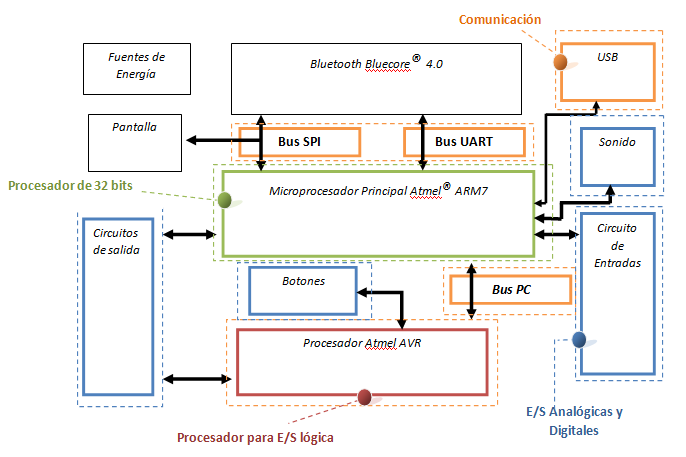
\includegraphics[width=\columnwidth]{diagramas/arquitectura-lego}
\caption{Arquitectura del SE del kit Lego NXT}
\label{fig:arquitectura-se-lego}
\end{figure}

El SE ha sido habilitado con un actuador (motor) que representa al compresor del aire acondicionado presente en el planteamiento del problema.

Además, se han incluido dos sensores de contacto que representan el botón de encendido - apagado de las luces, y el botón para permitir que el usuario confirme el encendido del aire acondicionado a pesar de que la ventana esté abierta.

Finalmente, se ha incorporado al SE un sensor de ultrasonido para fungir como sensor de presencia y un led para simular el encendido y apagado de las luces.

La configuración final del SE es mostrada en la Figura \ref{fig:configuracion-lego}.

\begin{figure}[!t]
\centering
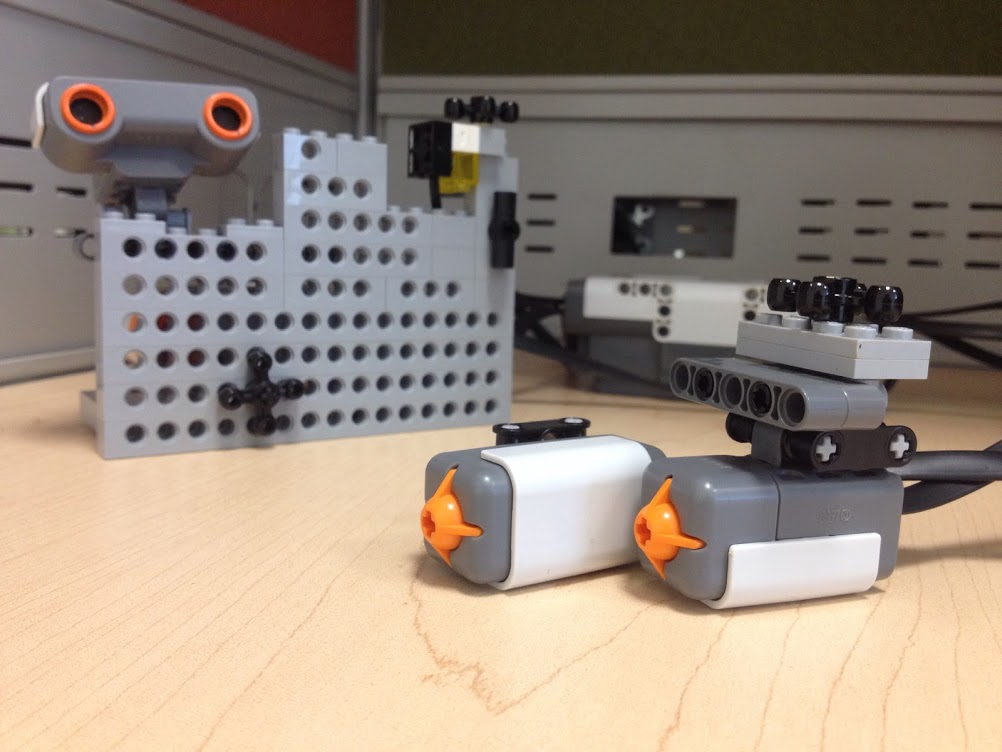
\includegraphics[width=\columnwidth]{diagramas/configuracion-lego2}
\caption{Configuración del kit Lego NXT}
\label{fig:configuracion-lego}
\end{figure}

\subsection{Descripción de la implementación}
\label{sub:metodologia-modelado-statechart}

La descripción de la implementación puede ser abordada en dos partes, la primera comprendiendo el diseño y modelado del problema y la segunda referente a la codificación del diseño creado.

%\vspace{0.5cm}
\textbf{\emph{Diseño del sistema}}

El diseño del sistema fue realizado contemplando las funcionalidades locales en cuatro estados.
En cada estado del sistema local, se hicieron las restricciones pertinentes tomando en cuenta la concurrencia e interacción con otros módulos.
Cada uno de estos estados, representa una situación en el sistema e internamente se encuentra a la escucha de una o más señales para desencadenar un comportamiento específico, seguido por la \emph{transición} a un nuevo estado.

La Figura \ref{fig:estados-modelo} muestra el diagrama de Statecharts general de los estados diseñados.
A grandes rasgos, cada uno de los estados describe en su interior un comportamiento similar al mostrado en la Figura \ref{fig:start}; y descrito a continuación:

	\begin{figure}
\centering
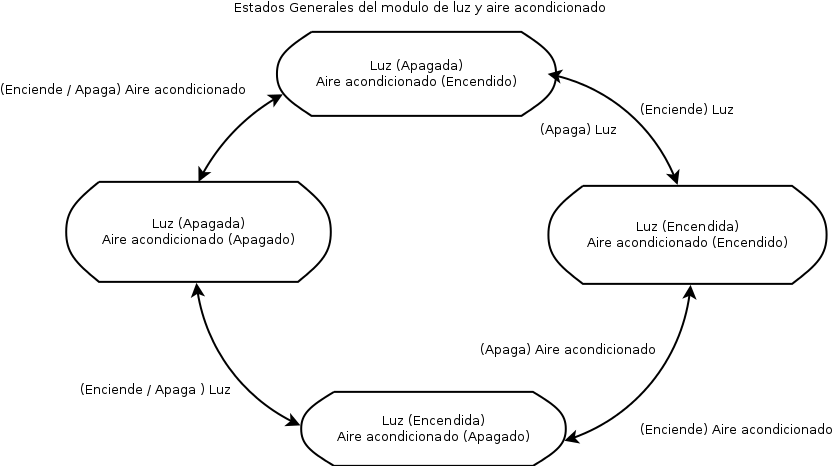
\includegraphics[width=\columnwidth]{diagramas/Diagrama_estados.png}
\caption{Diagrama global del módulo de luces y aire acondicionado.}
\label{fig:estados-modelo}
\end{figure}

	
%
\begin{itemize}
	\item \textbf{Inicial (Start) \ref{fig:start}:}
	En este estado se detecta un evento que indique una de las siguientes situaciones:
	\begin{itemize}
		\item El botón de encendido - apagado de la luz fue pulsado.
		\item El sensor de presencia no ha detectado movimiento en la habitación.
		\item Se ha recibido una configuración de horario para el funcionamiento de las luces y el aire acondicionado.
	\end{itemize}
\begin{figure}
\centering
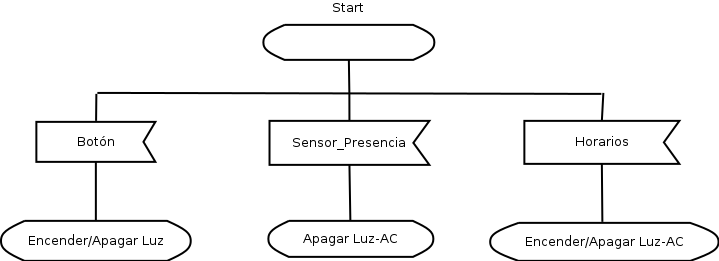
\includegraphics[width=\columnwidth]{diagramas/Diagrama_principal.png}
\caption{Start.}
\label{fig:start}
\end{figure}
\end{itemize}

Dicho estado inicial permite alcanzar otros estados internos que son descritos en los siguientes puntos.

\begin{itemize}

	\item  \textbf{Encender/Apagar Luz \ref{fig:estados1} :} La función principal de este estado es la de encender y apagar la luz.
	Es posible acceder a este estado, si el estado \emph{Start} detecta que fue presionado el botón touch que funciona como apagador de luz.
\begin{figure}
\centering
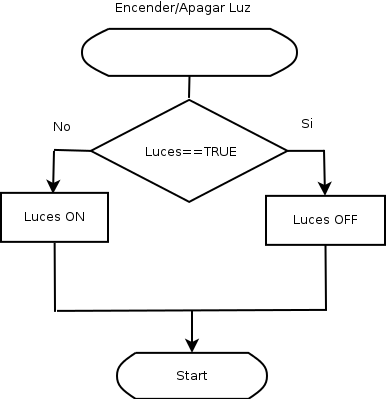
\includegraphics[width=\columnwidth]{diagramas/Encender_apagar_luz.png}
\caption{Encender/Apagar Luz.}
\label{fig:estados1}
\end{figure}
	\item  \textbf{Encender/Apagar AC \ref{fig:estados2} :} Este estado permite encender o apagar el aire acondicionado.
	Este estado es accesible a partir de los estados Apagar Luz-AC y Encender/Apagar Luz-AC.
	
	\begin{figure}
\centering
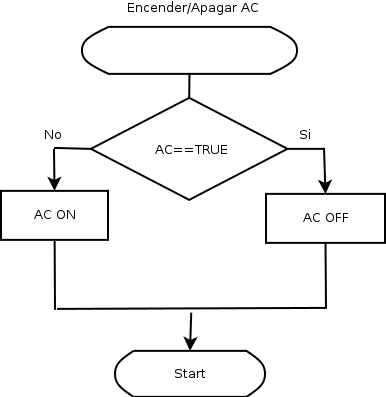
\includegraphics[width=\columnwidth]{diagramas/Encender_apagar_AC.png}
\caption{Encender/Apagar AC.}
\label{fig:estados2}
\end{figure}

	 \item \textbf{Encender/Apagar Luz-AC \ref{fig:estados3}:} Este estado se activa cuando el estado \emph{Start} detecta una configuración de horario, siendo posible realizar el encendido o apagado de la luz y del aire acondicionado.

\begin{figure}
\centering
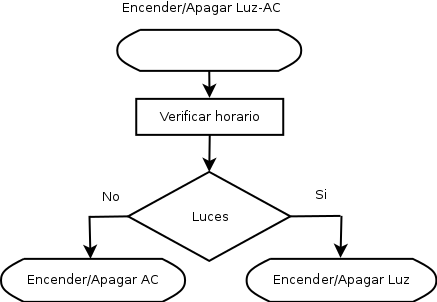
\includegraphics[width=\columnwidth]{diagramas/Encender_apagar_luz_AC.png}
\caption{Encender/Apagar Luz-AC.}
\label{fig:estados3}
\end{figure}	 
	 
	  \item \textbf{Apagar Luz-AC \ref{fig:estados4}:} Este estado es accesible sólo si el sensor de presencia no detecta movimiento dentro de la habitación.

	  Para realizarlo, el sensor debe obtener una distancia mayor a un umbral durante un umbral de tiempo determinado. Ambos umbrales son definidos por el sistema.
	  Cuando esto sucede, se determina que la habitación está vacía y por lo tanto se instruye el apagado de la luz y el aire acondicionado, en caso de estar encendidos.
\end{itemize} 

\begin{figure}
\centering
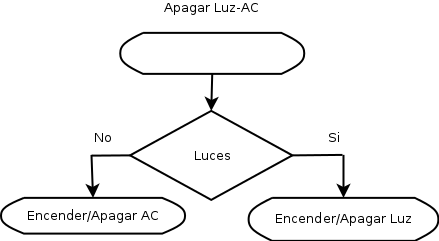
\includegraphics[width=\columnwidth]{diagramas/Apagar_luz_AC.png}
\caption{Apagar Luz-AC.}
\label{fig:estados4}
\end{figure}


%\vspace{0.5cm}
\textbf{\emph{Codificación del diseño}}

Debido a que la elaboración del diseño utilizando Statecharts se manifiesta como una máquina de estados finitos, el pseudocódigo de la implementación refleja un bucle infinito con un bloque \emph{switch} embebido, el cual contiene en cada uno de sus \emph{case’s} a los estados previamente descritos.

En Pseudocódigo \ref{alg:pseudocodigo} se muestra el pseudocódigo del SE, ilustrando el bloque \emph{switch} y la navegación entre sus estados.

Para poder responder ante las interacciones con los otros módulos (control de persianas y ventanas, control de puerta de acceso) se realizaron las validaciones pertinentes.
Gracias a ello, el sistema puede responder de forma inteligente al ambiente que lo rodea.
Para la interacción con los otros módulos, el sistema se apoya en la infraestructura de comunicación Bluetooth incluida en el Lego NXT, respondiendo y atendiendo a las peticiones hechas por parte de un agente externo al SE. 

\begin{algorithm}
\caption{Pseudocódigo de la implementación.}
\begin{algorithmic}[1]
\State{\textbf{Recibe:} Bóton,Sensor\_Presencia,Horario}
\State{\textbf{Retorna:} estadoLuz, estadoAC}
\State{Inicializar Sensores}
\State{estado=L-off\_AC-off}
  \Switch{estado}
  
    %caso 1
    \Case{L-off\_AC-off}
    %boton
    \If{Bóton}
     \If{Luz encendida}
    \State{apagar luces}
    \State{estado=L-off\_AC-off}
     \EndIf
      \If{Luz apagada}
    \State{encender luces}
    \State{estado=L-on\_AC-off}
     \EndIf
     \EndIf
     %horario
       \If{Horario}
     \If{Es tiempo de encender las luces}
    \State{encender luces}
    \State{estado=L-on\_AC-off}
     \EndIf
      \If{Es tiempo de apagar las luces}
    \State{encender luces}
    \State{estado=L-off\_AC-off}
     \EndIf
     \EndIf
       \If{Es tiempo de encender el aire acondicionado}
    \State{encender AC}
    \State{estado=L-off\_AC-on}
     \EndIf
      \If{Es tiempo de apagar el aire acondicionado}
    \State{encender AC}
    \State{estado=L-off\_AC-off}
     \EndIf
    
   %sensor  
        \If{Sensor\_Precencia}
     \If{No hay nadie en la habitación y (luz encendida o aire acondicionado encendido)}
   
      \If{Luz encendida}
    \State{apagar luces}
    \State{estado=L-off\_AC-off}
     \EndIf
         \If{Aire acondicionado encendido}
    \State{apagar AC}
    \State{estado=L-off\_AC-off}
    \EndIf
     \EndIf
     \EndIf
     
    \EndCase
    
     \algstore{bkbreak}
\end{algorithmic}
\end{algorithm}

\begin{algorithm}
\caption{Pseudocódigo de la implementación.}
\begin{algorithmic}[1]
\algrestore{bkbreak}
    \Case{L-off\_AC-on}
    \If{Bóton}
    
    
     \If{Luz encendida}
    \State{apagar luces}
    \State{estado=L-off\_AC-on}
     \EndIf
     
      \If{Luz apagada}
    \State{encender luces}
    \State{estado=L-on\_AC-on}
     \EndIf
     
     \EndIf
     
       \If{Horario}
       
     \If{Es tiempo de encender las luces}
    \State{encender luces}
    \State{estado=L-on\_AC-on}
     \EndIf
     
      \If{Es tiempo de apagar las luces}
    \State{encender luces}
    \State{estado=L-off\_AC-on}
     \EndIf
     
       \If{Es tiempo de encender el aire acondicionado}
    \State{encender AC}
    \State{estado=L-off\_AC-on}
     \EndIf
     
      \If{Es tiempo de apagar el aire acondicionado}
    \State{encender AC}
    \State{estado=L-off\_AC-off}
     \EndIf
     
     \EndIf
     
        \If{Sensor\_Precencia}
        
     \If{No hay nadie en la habitación y (luz encendida o aire acondicionado encendido)}
   
      \If{Luz encendida}
    \State{apagar luces}
    \State{estado=L-off\_AC-on}
     \EndIf
     
    \If{Aire acondicionado encendido}
    \State{apagar AC}
    \State{estado=L-off\_AC-off}
     \EndIf
     
     \EndIf
       \EndIf
     
    \EndCase
      %caso 3 
           \algstore{bkbreak}
\end{algorithmic}
\end{algorithm}

\begin{algorithm}
\caption{Pseudocódigo de la implementación.}
\begin{algorithmic}[1]
\algrestore{bkbreak}
  \Case{L-on\_AC-on}
    \If{Bóton}
     \If{Luz encendida}
    \State{apagar luces}
    \State{estado=L-off\_AC-on}
     \EndIf
      \If{Luz apagada}
    \State{encender luces}
    \State{estado=L-on\_AC-on}
     \EndIf
     \EndIf
     
       \If{Horario}
     \If{Es tiempo de encender las luces}
    \State{encender luces}
    \State{estado=L-on\_AC-on}
     \EndIf
      \If{Es tiempo de apagar las luces}
    \State{encender luces}
    \State{estado=L-off\_AC-on}
     \EndIf
       \If{Es tiempo de encender el aire acondicionado}
    \State{encender AC}
    \State{estado=L-on\_AC-on}
     \EndIf
      \If{Es tiempo de apagar el aire acondicionado}
    \State{encender AC}
    \State{estado=L-on\_AC-off}
     \EndIf
     \EndIf
     
        \If{Sensor\_Precencia}
     \If{No hay nadie en la habitación y (luz encendida o aire acondicionado encendido)}
   
      \If{Luz encendida}
    \State{apagar luces}
    \State{estado=L-off\_AC-on}
     \EndIf
         \If{Aire acondicionado encendido}
    \State{apagar AC}
    \State{estado=L-off\_AC-off}
     \EndIf
     \EndIf
        \EndIf
    \EndCase
        %caso 4
             \algstore{bkbreak}
\end{algorithmic}
\end{algorithm}

\begin{algorithm}
\caption{Pseudocódigo de la implementación.}
\begin{algorithmic}[1]
\algrestore{bkbreak}
    \Case{L-on\_AC-off}
    \If{Bóton}
     \If{Luz encendida}
    \State{apagar luces}
    \State{estado=L-off\_AC-off}
     \EndIf
      \If{Luz apagada}
    \State{encender luces}
    \State{estado=L-on\_AC-off}
     \EndIf
     \EndIf
     
       \If{Horario}
     \If{Es tiempo de encender las luces}
    \State{encender luces}
    \State{estado=L-on\_AC-off}
     \EndIf
      \If{Es tiempo de apagar las luces}
    \State{encender luces}
    \State{estado=L-off\_AC-off}
     \EndIf
       \If{Es tiempo de encender el aire acondicionado}
    \State{encender AC}
    \State{estado=L-on\_AC-on}
     \EndIf
      \If{Es tiempo de apagar el aire acondicionado}
    \State{encender AC}
    \State{estado=L-on\_AC-off}
     \EndIf
     \EndIf
     
        \If{Sensor\_Precencia}
     \If{No hay nadie en la habitación y (luz encendida o aire acondicionado encendido)}
   
      \If{Luz encendida}
    \State{apagar luces}
    \State{estado=L-off\_AC-off}
     \EndIf
         \If{Aire acondicionado encendido}
    \State{apagar AC}
    \State{estado=L-on\_AC-off}
     \EndIf
     \EndIf
       \EndIf

   \EndCase
    
  \EndSwitch
\end{algorithmic}
%\caption{Pseudocódigo de la implementación.}
\label{alg:pseudocodigo}
\end{algorithm}



\section{Resultados} 
\label{sec:resultados}
Después de la realización de pruebas con el sistema implementado, se han obtenido resultados satisfactorios, por lo que el sistema se comporta de acuerdo a lo establecido en los lineamientos iniciales.

Gracias a que el lego NXT cuenta con puertos de entrada y salida suficientes para simular el comportamiento de control de luces y aire acondicionado, los estados programados del sistema, se pudieron llevar a cabo sin ninguna complicación, esto para el funcionamiento local del sistema.

En cuanto a aspectos de domótica se refiere, el módulo de luces y aire acondicionado se adecua a su ambiente, enviando y recibiendo un flujo de datos que permite detectar los cambios y hacer validaciones en cada estado del sistema.

\section{Discusión y conclusiones}
\label{sec:discusion}
A pesar de la aparente sencillez de la actividad realizada de manera local, es importante notar que resultó un buen reto para mejorar las capacidades de diseño y modelado de SE, particularmente en entornos concurrentes que requieren comunicación con elementos externos al SE.

Debido a estos requerimientos, el diseño se realizó considerando que dentro del ambiente del Lego podrían existir otros módulos con los que se podría interactuar a través de un protocolo específico en tiempo real, detectando cambios en el entorno y realizando las adecuaciones pertinentes en su comportamiento.
 
La perspectiva del diseño de sistemas de este tipo es muy distinta a la observada en la construcción de \emph{software clásico}, ya que hay un especial interés en la obtención de los elementos que van a participar en el sistema y su interacción, a diferencia del software clásico en el que lo que normalmente se busca es la obtención e implementación de un algoritmo a modo de serie de pasos para lograr un requisito establecido desde el análisis.

Como un comentario final, nos ha parecido relevante el hecho de que después de contar el modelo y haber reconocido que la cobertura ante los escenarios descritos era la adecuada, la implementación (codificación) del SE se aceleró de forma considerable.

\begin{thebibliography}{00}

\bibitem{wi}
\url{http://es.wikipedia.org/wiki/Sistema_embebido}
\bibitem{}
\url{https://education.lego.com/da-dk/lesi/support/product-support/mindstorms-education-nxt/nxt-base-set-9797/building-instructions}
\bibitem{}
\url{http://dx.doi.org/10.1016/0167-6423(87)90035-9}
\bibitem{}
\url{http://www.lgi2p.ema.fr/~urtado/Papers/SEKE09.pdf}
\bibitem{}
\url{http://dl.acm.org/citation.cfm?id=1164052}
\bibitem{Burns2005}
A. Burns y A. Wellings, Sistemas de Tiempo Real y Lenguajes de Programación, ADDISON - WESLEY, 2005.

\end{thebibliography}
\end{document}
